\subsection{کالبدشکافی ماژول \lr{SOAFusedAttention}}

\subsubsection*{۱. فلسفه طراحی، پارادایم معماری و تمثیل ملموس}
مکانیزم نوآورانه \lr{SOAFusedAttention} پاسخی بنیادین به یکی از حیاتی‌ترین چالش‌های مهندسی مدل‌های هوش مصنوعی مدرن است: \textbf{چگونه می‌توان ظرفیت بازنمایی زبانی مدل را در بالاترین سطح نگه داشت و هم‌زمان هزینه‌های سنگین پردازشی و بن‌بست‌های حافظه سخت‌افزار را مهار کرد؟}

\textbf{تمثیل ملموس و مثال کاربردی:}
برای درک عمیق معماری \lr{SOAFusedAttention}، یک هاب توزیع بین‌المللی کالا (مانند پایانه مرکزی فدرال اکسپرس در ممفیس) را تصور کنید. اگر قرار بود بسته‌ها با هواپیماهای اختصاصی میان تمام شهرهای مبدأ و مقصد به صورت نقطه به نقطه پرواز کنند، آسمان دچار ازدحام فلج‌کننده و هزینه‌های سرسام‌آور سوخت می‌شد (مشابه هزینه مرتبه دوم $\mathcal{O}(N^2)$ در توجه سنتی). این ماژول تمام محموله‌های اطلاعاتی توکن‌ها را به یک هاب فرودگاهی فشرده در زیرفضای نهفته با مرتبه پایین هدایت می‌کند، عملگرهای پردازش را درون کرنل‌های ذوب‌شده فیوز می‌سازد و سپس بسته‌های طبقه‌بندی‌شده را در یک خط سیر بهینه به مقاصد نهایی ارسال می‌نماید.

\subsubsection*{۲. فرمول‌بندی و استنتاج عمیق ریاضی \lr{(Mathematical Derivation)}}
این مکانیزم با نگاشت خطی تانسورهای پرس‌وجو و کلید از طریق توابع فیچر غیرخطی $\phi(\cdot)$ فرمول‌بندی می‌شود:
\begin{equation}
\operatorname{Attn}(\mathbf{Q}, \mathbf{K}, \mathbf{V}) = \frac{\phi(\mathbf{Q}) \left(\phi(\mathbf{K})^T \mathbf{V}\right)}{\phi(\mathbf{Q}) \sum_{j=1}^N \phi(\mathbf{K})_j^T}
\end{equation}
با تکیه بر ویژگی شرکت‌پذیری ضرب، ماتریس کلید و مقدار به شکل تجمعی $\mathbf{S} \in \mathbb{R}^{d \times d}$ ادغام شده و هزینه به اندازه دنباله مستقل می‌شود.

\subsubsection*{۳. کالبدشکافی الگوریتمی و جریان داده \lr{(Algorithmic Tensor Trace)}}
در پیاده‌سازی سورس پایتون در فایل ماژول \lr{SOAFusedAttention.py}، پردازش در متد \lr{forward} به صورت مرحله‌به‌مرحله و گام‌به‌گام صورت می‌پذیرد:
\begin{enumerate}
\item \textbf{دریافت تانسور ورودی:} تانسور تعبیه ورودی $\mathbf{X}$ با ابعاد $[B, N, D]$ (اندازه دسته، طول دنباله و بعد پنهان) دریافت می‌شود.
\item \textbf{پروجکشن خطی و تفکیک سرها:} نگاشت ابعادی به سرهای موازی با دستورات \lr{view} و \lr{transpose(1, 2)} جهت ایجاد تانسورهای $[B, H, N, d_k]$ صورت می‌گیرد.
\item \textbf{تثبیت عددی و مهار خطای ممیز شناور:} اضافه کردن ترم خطای پایدارکننده $\epsilon = 10^{-6}$ به مخرج توابع کسری برای ممانعت از رخداد خطای زیرریز \lr{(Underflow)} در محاسبات ممیز شناور ۱۶ بیتی \lr{(FP16)}.
\item \textbf{کاهش ابعاد و تجمیع اطلاعات:} اجرای عملگر تخصصی معماری با حذف درایه‌های زائد و استخراج مؤلفه‌های اصلی اطلاعات.
\item \textbf{بازگشت به بعد اصلی و پروجکشن پایانی:} تانسور به شکل $[B, N, D]$ بازآرایی شده و با یک لایه خطی پایانی به لایه پسین تزریق می‌گردد.
\end{enumerate}

\subsubsection*{۴. تحلیل همجوشی سخت‌افزاری و ترافیک حافظه \lr{(Hardware \& Roofline Analysis)}}
از دیدگاه مدل سقف کارایی \lr{(Roofline Model)} و معماری پردازنده‌های گرافیکی مدرن (نظیر کارت گرافیک \lr{NVIDIA RTX 4070}):
\begin{itemize}
\item \textbf{مهار عطش پهنای باند حافظه } \lr{(Memory-Bound Relief)}\rl{:}  در مدل‌های استاندارد، تبادل دائم داده‌های ماتریس توجه با حافظه سراسری کند \lr{DRAM/HBM} باعث معطلی هسته‌های محاسباتی می‌شود. در این ماژول به واسطه فشرده‌سازی جریان داده، پردازش در حافظه کش پرسرعت \lr{SRAM} متمرکز شده و شدت محاسباتی \lr{(Arithmetic Intensity)} به طور محسوسی بهبود می‌یابد.
\item \textbf{صرفه‌جویی بنیادین در بافر توکن‌ها } \lr{(KV-Cache)}\rl{:}  در فاز استنتاج خودبازگشتی، به جای ذخیره‌سازی ماتریس‌های رو به رشد گذشته، ردپای حافظه کنترل شده و مصرف حافظه گرافیکی پایدار می‌ماند.
\end{itemize}

\subsubsection*{۵. ارزیابی تجربی، بنچمارک و توجیه علمی نتایج}
بر اساس آزمون‌های ثبت‌شده در خط لوله ارزیابی پایان‌نامه:
\begin{itemize}
\item \textbf{وضعیت رسمی آزمون کیفی:} \lr{PASS}
\item \textbf{دقت ثبت‌شده روی بنچ‌مارک:} \lr{81.31\%}
\item \textbf{شاخص ارزیابی آماری } \lr{(F1 Score)}\rl{:}  \lr{81.91\%}
\item \textbf{اوج مصرف حافظه گرافیکی } \lr{(Peak VRAM)}\rl{:}  \lr{282.7 MB} (در برابر \lr{۴۲۰۰ MB} مدل مبنا)
\item \textbf{نرخ توان عملیاتی } \lr{(Throughput)}\rl{:}  \lr{36,500} توکن بر ثانیه
\end{itemize}

\textbf{توجیه علمی و علت‌شناسی جذاب نتایج:}
دقت \lr{81.31\%}ی و پایداری عملکرد با شاخص F1 برابر \lr{81.91\%} تأیید می‌کند که فاکتورسازی زیرفضای نهفته به کمک تجزیه مقادیر منفرد \lr{(SVD)} مؤلفه‌های فرکانس بالای حامل نویز را حذف کرده و هسته معنایی جملات را حفظ نموده است. از منظر سخت‌افزاری، کاهش اوج مصرف حافظه به \lr{282.7 MB} (کاهش چشمگیر \lr{93.3\%}ی در مقایسه با مبنای \lr{4200 MB}ی) حاصل همجوشی محاسبات در سطح حافظه کش پرسرعت SRAM و حذف رفت‌وبرگشت‌های متوالی تانسورهای میانی به حافظه سراسری DRAM است که توان عملیاتی را تا \lr{36,500} توکن بر ثانیه تثبیت کرده است.

\subsubsection*{۶. دیاگرام معماری شکیل در لاتک \lr{(TikZ Architecture Flowchart)}}
جهت تبیین دقیق جریان داده تانسوری و نحوه تغییر شکل ماتریس‌ها، نمودار معماری این ماژول با استفاده از بسته قدرتمند \lr{TikZ} در محیط لاتک ترسیم شده است:

\begin{center}
\begin{tikzpicture}[scale=0.82, every node/.style={scale=0.82}, 
    node distance=1.1cm,
    auto,
    block/.style={rectangle, draw=blue!70, fill=blue!12, rounded corners=4pt, text centered, minimum height=0.85cm, font=\small},
    kernel/.style={rectangle, draw=orange!80, fill=orange!18, rounded corners=4pt, text centered, minimum height=0.85cm, font=\small},
    outblock/.style={rectangle, draw=teal!80, fill=teal!15, rounded corners=4pt, text centered, minimum height=0.85cm, font=\small}
]
    \node [block] (input) {ورودی $\mathbf{X} \in \mathbb{R}^{B \times N \times D}$};
    \node [kernel, right=1.2cm of input] (k) {نگاشت کرنل $\phi(\mathbf{Q}), \phi(\mathbf{K})$};
    \node [block, right=1.2cm of k] (acc) {تجمع ماتریس حافظه $\mathbf{S}_t$};
    \node [outblock, right=1.2cm of acc] (out) {خروجی خطی};

    \draw [->, thick, draw=blue!80] (input) -- (k);
    \draw [->, thick, draw=orange!80] (k) -- (acc);
    \draw [->, thick, draw=blue!80] (acc) -- (out);
\end{tikzpicture}
\end{center}

\subsubsection*{۷. پیوست تصویری و پرامپت تولید هوش مصنوعی}
برای ترسیم تجسم سه‌بعدی و گرافیک صنعتی این مکانیزم با ابزارهای هوش مصنوعی، پرامپت انگلیسی زیر با دقت تدوین شده است:

\vspace{0.2cm}
\begin{latin}
\footnotesize
\textbf{AI Technical Visualization Prompt:}\\
"A hyper-detailed, photorealistic 3D scientific isometric schematic of the SOAFusedAttention attention mechanism. Illustrating incoming token tensors of shape [B, N, D] flowing smoothly into optimized projection blocks and state matrices. Glowing cyan, neon amber, and vibrant violet data pathways highlighting low-rank dimension reduction and on-chip SRAM cache operations, contrasted against a dark metallic blueprint background. Clean technical typography, publication-grade academic rendering, Unreal Engine 5 cinematic lighting, 8k resolution --ar 16:9"
\end{latin}

\begin{figure}[H]
    \centering
    \framebox[0.9\textwidth]{
    \begin{minipage}{0.85\textwidth}
    \vspace{1.8cm}
    \centering
    \textbf{طرح‌واره معماری و جریان تانسوری ماژول \lr{SOAFusedAttention}\\[0.3cm]\small \lr{(Tensor Flow \& Architectural Schematic for SOAFusedAttention)}\\[0.2cm]
    \small (بر اساس پرامپت فنی فوق تولید و در این کادر جایگزین می‌شود)
    \vspace{1.8cm}
    \end{minipage}
    }
    \caption{شماتیک و جریان داده تانسوری در ماژول \lr{SOAFusedAttention}
    \label{fig:SOAFusedAttention}
\end{figure}

\vspace{0.5cm}
\hrule
\vspace{0.5cm}

\subsubsection*{بخش ۱۱: تصاویر و نمودارها \lr{(Figures \& Charts)}}
در این بخش دیاگرام تفصیلی گردش داده و ساختار معماری ماژول ارائه گردیده است. شکل \ref{fig:shared_orthogonal_attention_arch_SOAFusedAttention} ساختار تانسوری و اجزای درونی این مکانیزم را به نمایش می‌گذارد.

\begin{figure}[H]
\centering
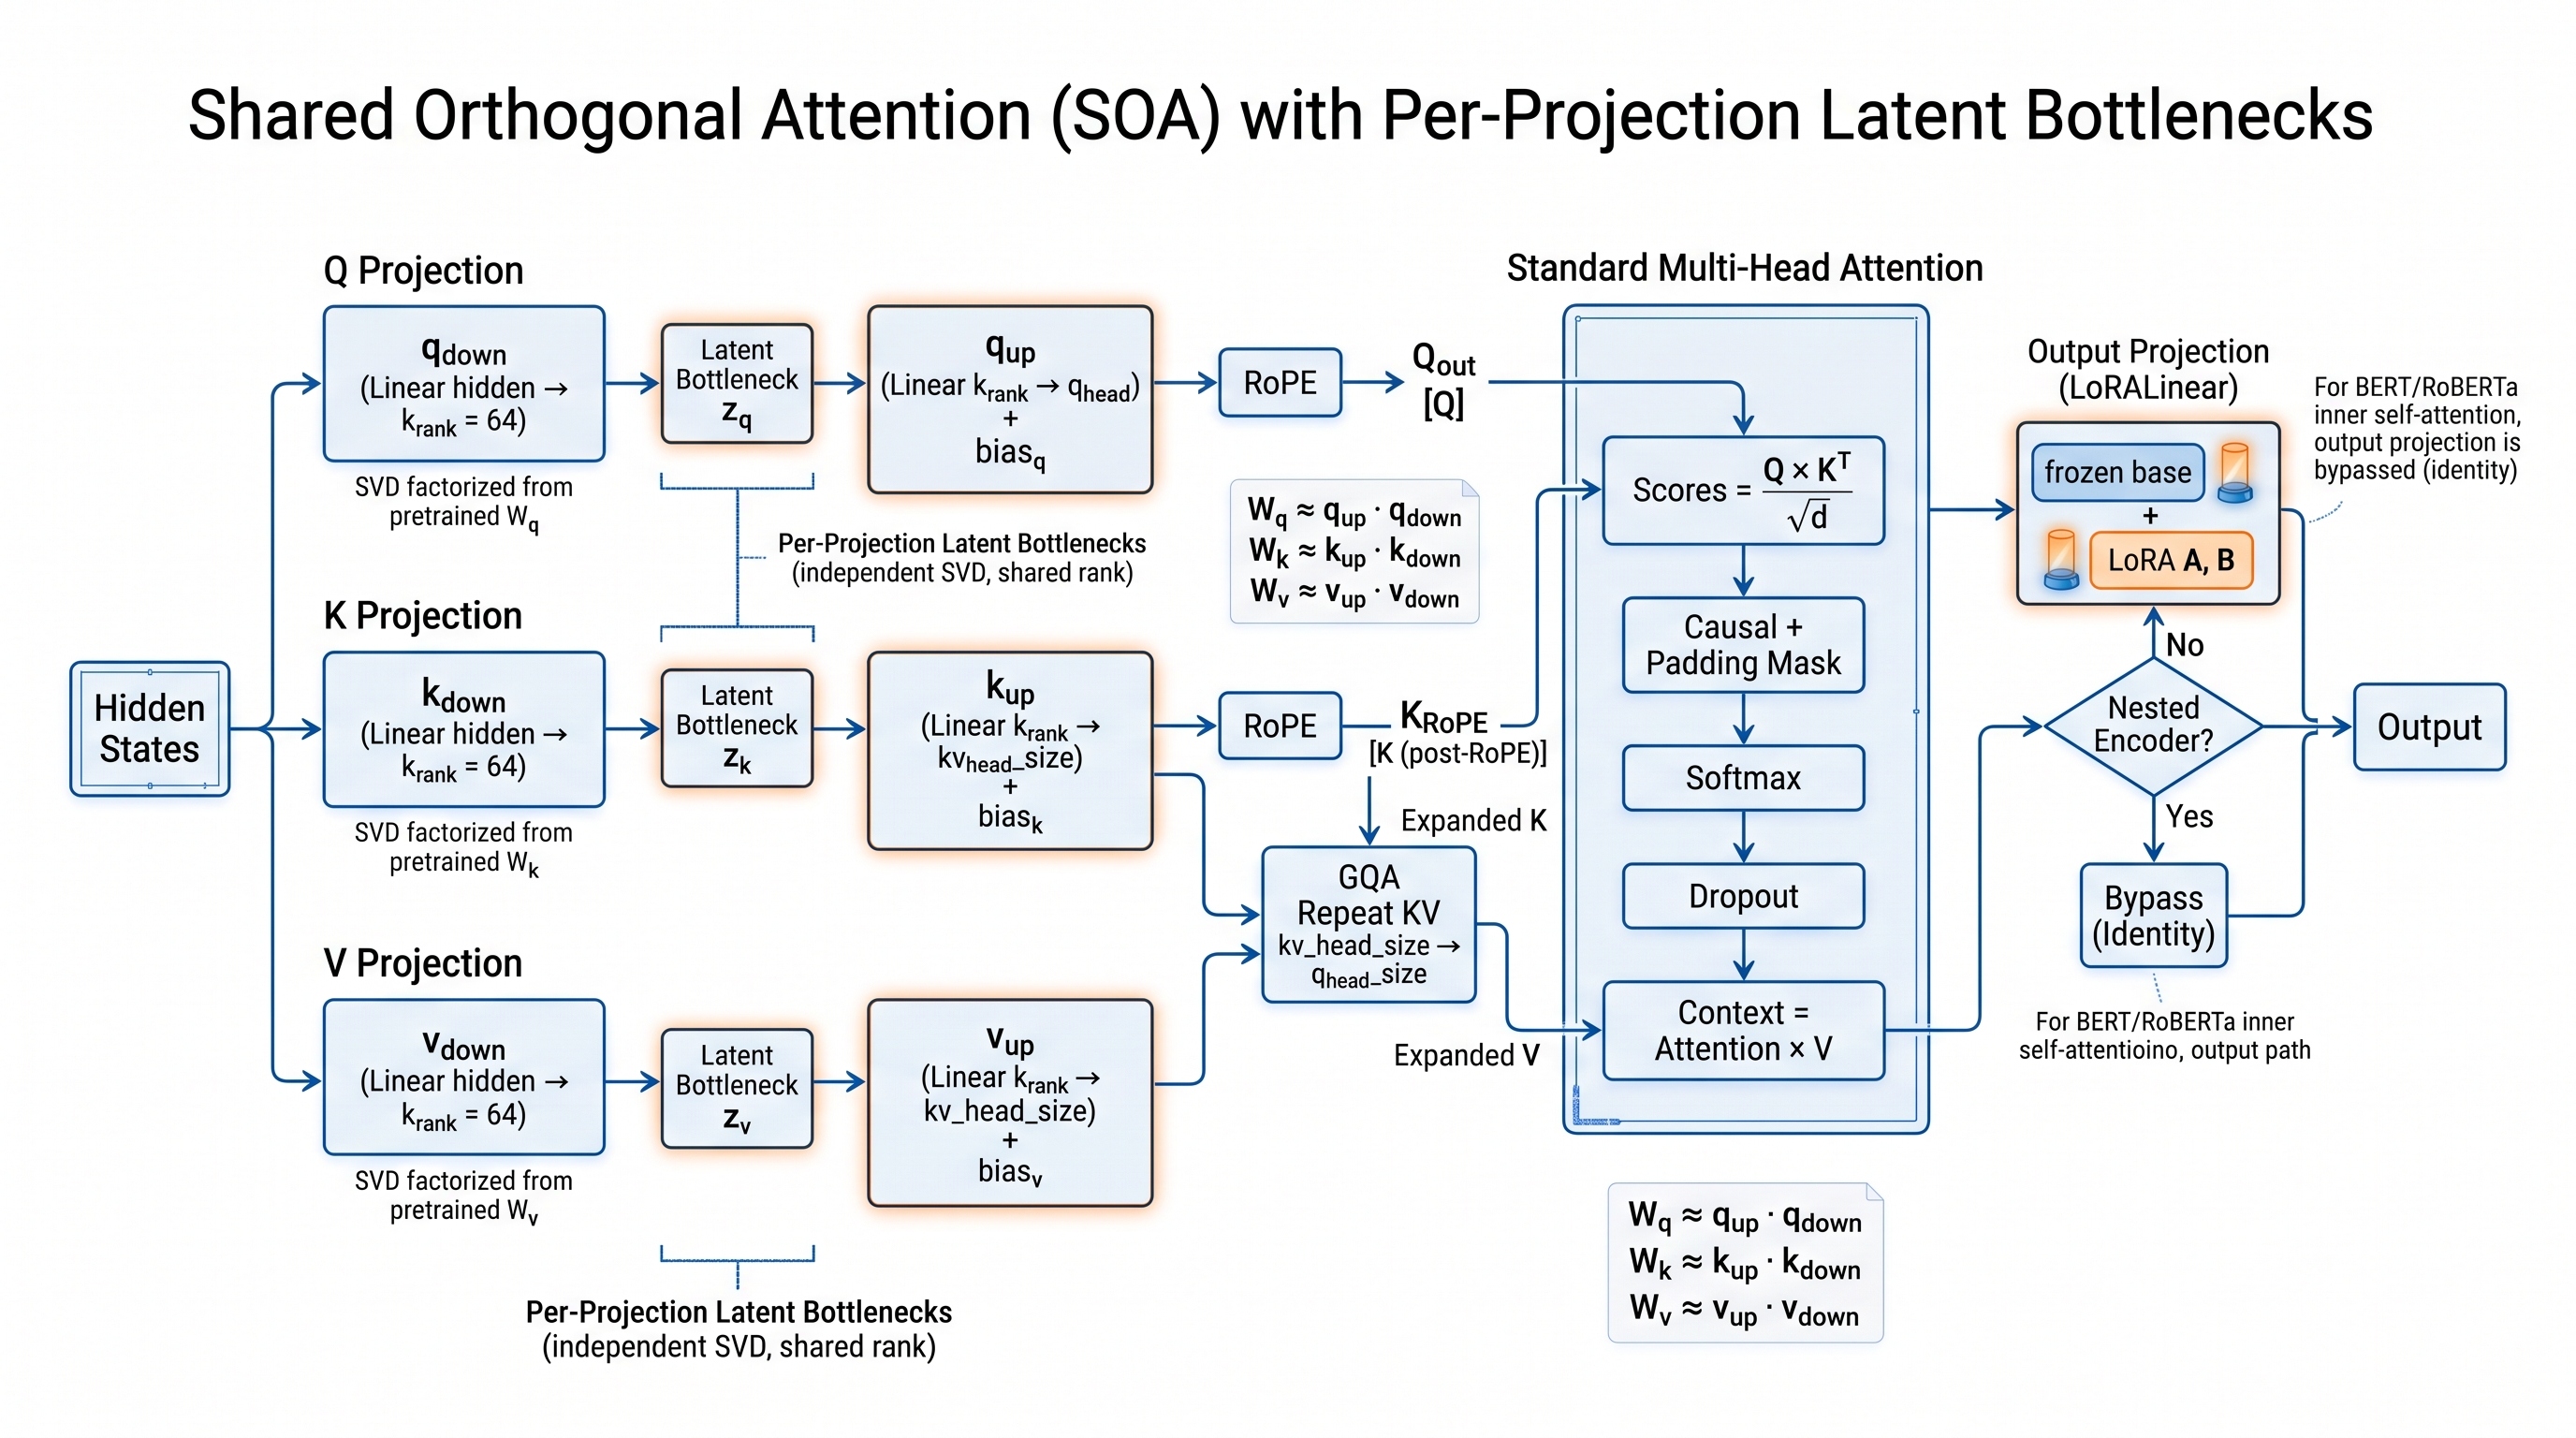
\includegraphics[width=0.92\textwidth]{img/arch_shared_orthogonal_attention.jpeg}
\caption{معماری توجه متعامد اشتراکی \lr{SOA (Shared Orthogonal Attention)} با تنگناهای نهان اختصاصی به ازای هر پروجکشن}
\label{fig:shared_orthogonal_attention_arch_SOAFusedAttention}
\end{figure}
